
In this section the focus is in the \textbf{Decoder Component implementation}. It is the group's specific component and so deserves to be explained with some detail. Until now, almost everything that was illustrated in this report has a certain importance and had an influence in the implementation that is about to be presented.

Summing up, the major steps were: the creation of the \textbf{\textit{EL} script} (\textit{.el} file) of this component,\textbf{ annotate the source} files and build the \textbf{elaboration files} according to each decoder behavior. 

\subsubsection{\textit{EL} script}

The moment of creation of the \textit{.el} file was a quite trivial step because it was based on the conceptual model. So, all that was needed was "translate" that conceptual model into \textit{EL} code. However, to be done so, it had to be \textbf{ensured that the theoretical model was perfectly well design}. In listing \ref{lst:EL_Decoder} it is represented the \texttt{Decoder.el} file, containing the \textit{EL} code that models this component.

\begin{lstlisting} [language=EL, caption=Decoder (EL representation), label=lst:EL_Decoder]
import "Languages.el"
import "Interfaces.el"

component Decoder (C)
{
      properties:
      			bool srcCodeTracing : true
      services:
      			i_Decode s_Decode
      references:
        i_ISA r_ISA
        i_Registers r_Registers
        i_SrcEnv r_SrcEnv
        i_Generate r_Generate
        i_CCache r_CCache
        i_EngineState r_EngineState
}
\end{lstlisting}

As it can be seen, it was defined the \textbf{property} \texttt{srcCodeTracing} which will be a configurable parameter. Also, the \textbf{service} and the \textbf{references} that were planned in the conceptual model were defined.


\subsubsection{Generated Files}

Compiling the top-level component, \texttt{DBT.el}, all the others \textit{.el} files are compiled too. As explained, a several number of intermediate and crucial files are generated. However, only the ones related to the decoder, and the more important ones, will be shown. Figure \ref{fig:decoder_xml} illustrates the location of the configuration file of the decoder, \texttt{decoder.xml}.

\begin{figure}[H]
\centerline{
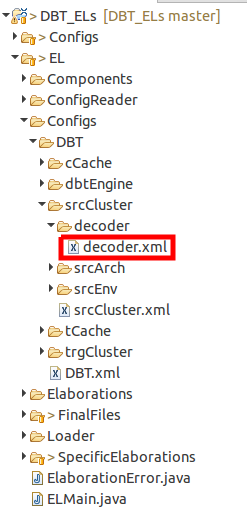
\includegraphics[scale=0.38]{images/decoder}
}
\caption{Location of the \texttt{decoder.xml} file.}
\label{fig:decoder_xml} 
\end{figure}

It's possible to verify the good organization of the files in the folders, i.e., the chain of folders are disposed in a way that allows to keep a consistence with the disposition of the components in the model. This way, its easier to navigate through the file system.

\begin{figure}[H]
\centerline{
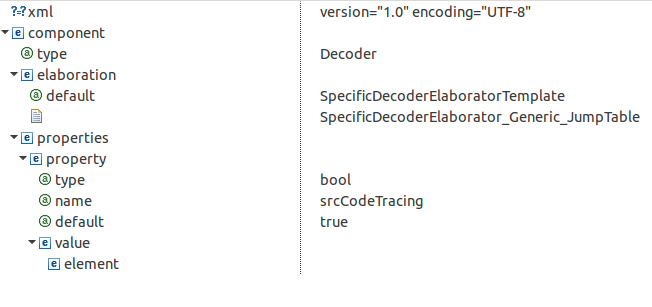
\includegraphics[scale=0.38]{images/decoder2}
}
\caption{\texttt{decoder.xml} file.}
\label{fig:decoder_xml2} 
\end{figure}
 
It is represented, in figure \ref{fig:decoder_xml2}, the \texttt{decoder.xml} file. It is in this file that the elaboration file is chosen, on the \textbf{\textit{<elaboration>} field} in the \texttt{xml}, and that the configuration of the property (\texttt{srcCodeTracing}) is made by the user, on the\textit{\textbf{ <property>}} field. By default, this property has the value \textbf{true} (bool).

Besides the configurations folder, another crucial one is created, the decoder specific elaborations folder (figure \ref{fig:decoder_spec}).

\begin{figure}[H]
\centerline{
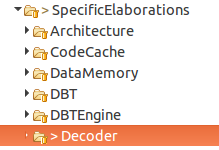
\includegraphics[scale=0.5]{images/decoder3}
}
\caption{\texttt{Decoder specific elaboration folder} file.}
\label{fig:decoder_spec}
\end{figure}

After compilation, it is created, in the decoder specific elaborations folder, a template elaboration file to guide the designer. From there, his role is to create specific elaboration files and put them in specific folders along with the specific annotated sources (if they are not shared between other components elaborations). The specific elaboration files will be discussed right ahead, in the next section.

\subsubsection{Elaboration Files}

Despite the behaviors implemented, only the ones purely in software were integrated with the global system (\textit{DBT}). Later it will be discussed the reason for that event. 

This section presents one of the roles of the designer, \textbf{the creation of the specific elaboration files}. As mentioned, since the "existence" of three possible behaviors, an specific elaboration file to each must be done. To achieve that, the first step was the creation of \textbf{three specific folders} in the decoder specific elaborations folder. It is possible to observe the first step in figure \ref{fig:decoder_spec2}.

\begin{figure}[H]
\centerline{
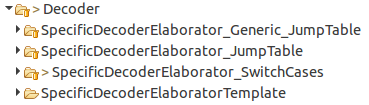
\includegraphics[scale=0.5]{images/spec1}
}
\caption{Decoder specific elaborations folders.}
\label{fig:decoder_spec2}
\end{figure}

Besides the specific elaboration files, it must be also known the files that need to be filled with annotations, to be placed in the specific folders. It can be already revealed that the only files that need to be "manipulated" by the decoder are the \texttt{SourceArch\_8051.cpp}, the \texttt{SourceArch\_8051.h} and the \texttt{types.h}. Yet, the \texttt{SourceArch\_8051.h} and the  \texttt{types.h} are also modified by elaboration files of other components and so, they must be placed in the \textit{SharedSources} folder (figure \ref{fig:decoder_spec3}). The \texttt{SourceArch\_8051.cpp} is exclusive to the decoder. Figure \ref{fig:decoder_spec4} illustrates the the decoder specific elaborations folder more composed.

\begin{figure}[H]
\centerline{
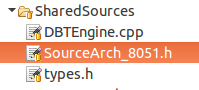
\includegraphics[scale=0.6]{images/spec2}
}
\caption{\textit{SharedSources} folder.}
\label{fig:decoder_spec3}
\end{figure}


\begin{figure}[H]
\centerline{
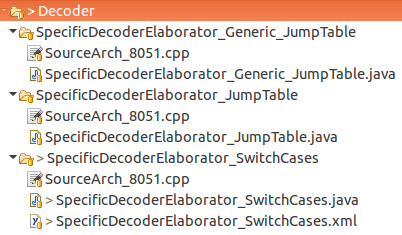
\includegraphics[scale=0.5]{images/spec3}
}
\caption{More composed decoder specific elaborations folder}
\label{fig:decoder_spec4}
\end{figure}

The annotation in the \texttt{types.h} file is related to the configurable property of the decoder component (listing \ref{lst:annot}). Depending on the value of the property, the annotation will be replaced with "//" to comment the define or will be replaced with "" keeping in the code the definition of the \texttt{SrcCodeTrace} MACRO.

\begin{lstlisting} [language=C++, caption=\texttt{types.h} file annotation.
, label=lst:annot]
@@Decoder_tracing@@#define SrcCodeTrace
\end{lstlisting}

As to the \texttt{SourceArch\_8051.h} file, since that it is placed in the \textit{SharedSources} folder, and so each decoder elaboration file will modify this same header file, the annotations were placed aiming the possible alterations of the three behaviors. So, if an elaboration just replace one annotation, the other annotations will be replaced with an empty value (""). Listing \ref{lst:annot2} shows the annotations placed in the \texttt{SourceArch\_8051.h} file.

\begin{lstlisting} [language=C++, caption=\texttt{SourceArch\_8051.h} file annotations.
, label=lst:annot2]

@@Decoder_Defines@@

...

@@Decoder_Variables@@

...

@@Decoder_Inits@@

...

@@Decoder_Methods@@ 

};
\end{lstlisting}


Independently of the behavior, the references of the decoder to services of other components are the same. So, what was done was go through each specific \texttt{SourceArch\_8051.cpp} file and place annotations in locations where the services are needed. Recalling, the decoder need services from the following components: the \textbf{Generator}, the \textbf{Source Environment}, the \textbf{Code Cache}, the \textbf{DBT Engine}. Listings \ref{lst:annot3}, \ref{lst:annot4}, \ref{lst:annot5} shows a fragment of the \texttt{SourceArch\_8051.cpp} file annotated, to each behavior.


\begin{lstlisting} [language=C++, caption=Fragment of the \texttt{SourceArch\_8051.cpp} file for the Switch cases behavior.
, label=lst:annot3]
@@Decoder_SwitchCases@@

...

void  C8051Arch::fineDecode_0x1(uint8_t subOp, uint8_t Rn){	// AJMP
			uint8_t tmp1;
			uint16_t newPC; 

			tmp1 = @@Decoder_Fetch@@;
			newPC = (env.@@Decoder_getPC@@ & 0xF800) | 0x0000 | (uint16_t)tmp1; 
  	target->@@Decoder_gen_writePC@@(newPC);	
  	zprintf("\tAJMP 0x%04X\n\n", newPC);
			*@@Decoder_eoBB@@ = true;		
}
\end{lstlisting}

\begin{lstlisting} [language=C++, caption=Fragment of the \texttt{SourceArch\_8051.cpp} file for the Jump Table behavior.
, label=lst:annot4]
void  C8051Arch::fineDecode_0x83(uint8_t subOp, uint8_t Rn){   // MOVC A, @A+PC
			target->@@Decoder_gen_ld8@@(tReg1, A);
			target->@@Decoder_gen_movi@@(tReg2, env.@@Decoder_getPC@@);
			target->@@Decoder_gen_add@@(tReg1, tReg1, tReg2);
		
			target->@@Decoder_gen_movi@@(tReg2, (int)@@Decoder_pSourceProgMem@@ );
			target->@@Decoder_gen_ldi8@@(tReg1, tReg2, tReg1 );
			target->@@Decoder_gen_st8@@( A, tReg1 );

			zprintf("\tMOVC A, @A+PC\n\n");
}
\end{lstlisting}

\begin{lstlisting} [language=C++, caption=Fragment of the \texttt{SourceArch\_8051.cpp} file for the Generic behavior.
, label=lst:annot5]
void C8051Arch::gen_cje_wrapper(arg_P * ptr){ 
    target->@@Decoder_gen_cje@@(*(uint8_t*)ptr[0], *(uint8_t*)ptr[1], *(uint8_t*)ptr[2]);    
}

void C8051Arch::gen_cjne_wrapper(arg_P * ptr){ 
    target->@@Decoder_gen_cjne@@(*(uint8_t*)ptr[0], *(uint8_t*)ptr[1], *(uint8_t*)ptr[2]);      
}

void C8051Arch::gen_cjei_wrapper(arg_P * ptr){
    target->@@Decoder_gen_cjei@@(*(uint8_t*)ptr[0], *(uint8_t*)ptr[1], *(uint8_t*)ptr[2]);    
}
\end{lstlisting}

Now, the process for replace some of the annotations are the same for the three specific elaborations. So, first it will be presented the commonalities and then more specific points. 

What is common to each elaboration is the replacement of the annotations of the references to services. Listing \ref{lst:annot6} shows the process of those replacements.

\newpage
\begin{lstlisting} [language=C++, caption=Common process of replacement.
, label=lst:annot6]
openAnnotatedSource("SourceArch_8051.cpp");   
		
//**************************GENERATOR INTERFACE*********************************
_Generator comp = (_Generator) target.get_r_Generate();
AbstractGeneratorElaborator GeneratorElab = (AbstractGeneratorElaborator) getElaborator(comp);
        
replaceAnotation("Decoder_gen_mov", (String) GeneratorElab.getI_GenerateElaboratorGen_mov());
replaceAnotation("Decoder_gen_movi", (String) GeneratorElab.getI_GenerateElaboratorGen_movi());
replaceAnotation("Decoder_gen_ld8", (String) GeneratorElab.getI_GenerateElaboratorGen_ld8());
replaceAnotation("Decoder_gen_ld16", (String) GeneratorElab.getI_GenerateElaboratorGen_ld16());
replaceAnotation("Decoder_gen_ldi8", (String) GeneratorElab.getI_GenerateElaboratorGen_ldi8());

			...

//**********************SOURCE ENVIRONMENT INTERFACE************************				
_SourceEnv SourceEnv_comp = (_SourceEnv) target.get_r_SrcEnv();
AbstractSourceEnvElaborator SourceEnvElab = (AbstractSourceEnvElaborator) getElaborator(SourceEnv_comp);
		
replaceAnotation("Decoder_getPC", (String) SourceEnvElab.getI_SrcEnvElaboratorGetPC());	
				
//****************************CODE CACHE INTERFACE*****************************/
_CodeCache CodeCache_comp = (_CodeCache) target.get_r_CCache();
AbstractCodeCacheElaborator CodeCacheElab = (AbstractCodeCacheElaborator) getElaborator(CodeCache_comp);
		
replaceAnotation("Decoder_Fetch", (String) CodeCacheElab.getI_CCacheElaboratorFetch());	
			
//**************************DBT ENGINE INTERFACE************************/	
_DBTEngine DBTEngine_comp = (_DBTEngine) target.get_r_EngineState();
AbstractDBTEngineElaborator DBTEngineElab = (AbstractDBTEngineElaborator) getElaborator(DBTEngine_comp);		
		
replaceAnotation("Decoder_eoBB", (String) DBTEngineElab.getI_EngineStateElaboratorEoBB());
replaceAnotation("Decoder_eoExec", (String) DBTEngineElab.getI_EngineStateElaboratorEoExec());
replaceAnotation("Decoder_pSourceProgMem", (String) DBTEngineElab.getI_EngineStateElaboratorPSourceProgMem());
    
//*************************DECODER TRACING PROPERTY*******************************/
		openAnnotatedSharedSource("types.h");
		if(target.get_srcCodeTracing()==true)
			replaceAnotation("Decoder_tracing","");
		else
			replaceAnotation("Decoder_tracing","//");	
\end{lstlisting}

Based on the listing above, it is firstly required to open the annotated source file using the \texttt{openAnnotatedSource()} function from the Elaboration \textit{API}, in this case, the \texttt{SourceArch\_8051.cpp}. Then, it is necessary to get the component that provides the service, in order to get its elaboration file, and replace the proper annotation according to specific service of that component, using the \texttt{replaceAnotation()} function. As to the replacement of the annotation that depends on the property \texttt{srcCodeTracing} of the Decoder, it is required to get the value of the property using getters functions(\texttt{target.get\_srcCodeTracing()}) of the class of the Decoder component.

As referred before, the decoder based on Switch cases has a point of configuration, which is the number of bits for the evaluation of the switch cases. Being those parameters specific to the behavior, an additional \texttt{XML} file must be created an placed in the specific folder (figure \ref{fig:decoder_spec10}).

\begin{figure}[H]
\centerline{
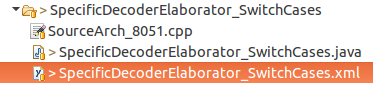
\includegraphics[scale=0.5]{images/spec10}
}
\caption{Additional \texttt{XML} file}
\label{fig:decoder_spec10}
\end{figure}

That being said, what was done in the specific elaboration file of the switch cases behavior was get from the additional \texttt{XML} the values of the properties, check some conditions and replace the annotation (listing \ref{lst:annot7}) with the generation of switch cases. It is possible to verify the process in the listing \ref{lst:annot8}.

\begin{lstlisting} [language=C++, caption=Algorithm to check the properties values and to replace the annotation.
, label=lst:annot8]
//***************************GENERATE SWITCH CASES***************************/			
		scr = getSpecificReader();
		int n1 = (Integer)scr.getProperty("n1");
		int n2 = (Integer)scr.getProperty("n2");
		
		if((n1 + n2) != nBitsOpcode || n1 < 0  || n2 < 0 || n1 > nBitsOpcode || n2 > nBitsOpcode)
		{
			ElaborationError.elaborationError("SWITCH CASES DECODER ERROR !!! --> The sum of the number of bits of each Switch Case must be equal to the number of bits of the opcode (8 bits)");
		}
		else
		{
			replaceAnotation("Decoder_SwitchCases",generateSwitchJmps(n1, n2));
		}
\end{lstlisting}

The role of the function \texttt{generateSwitchJmps()} is to, based on the configurable parameters, perform \texttt{for} loops and add to a string the code corresponding to the switch cases. That string is returned to the function \texttt{replaceAnotation()} and it will be the content for the annotation.

\begin{lstlisting} [language=C++, caption=Annotation in the \texttt{SourceArch\_8051.cpp} file of the Switch Cases decoder.
, label=lst:annot7]
@@Decoder_SwitchCases@@
\end{lstlisting}


Finally, the replacement of the annotations in the \texttt{SourceArch\_8051.h} file are different to each specific decoder elaboration, because it depends on the behavior. Therefore, it was necessary to insert \textbf{common annotations} and \textbf{specific ones}. So, all the elaborations modify the common annotations while the specific annotations are only modified by the respective elaboration. First lets check the replacement process for the Switch cases behavior (listing \ref{lst:annot9}).

\begin{lstlisting} [language=C++, caption=Annotations replacement process in the \texttt{SourceArch\_8051.h} (Switch Case Elaboration)
, label=lst:annot9]
openAnnotatedSharedSource("SourceArch_8051.h");

replaceAnotation("Decoder_Methods",generateCallBackFunction());
replaceAnotation("Decoder_Variables","");
replaceAnotation("Decoder_Defines","");
replaceAnotation("Decoder_Inits","");
\end{lstlisting}

As it can be seen, the switch cases specific elaboration file only replaces the \texttt{Decoder\_Methods} annotation, replacing the other annotations with an empty value (""). The \texttt{generateCallBackFunction()} function is responsible to generate a specific portion code correspondent to the behavior and return it as a string. As to the Jump Table decoder: 

\begin{lstlisting} [language=C++, caption=Annotations replacement process in the \texttt{SourceArch\_8051.h} (Jump Table Elaboration)
, label=lst:annot10]
openAnnotatedSharedSource("SourceArch_8051.h");
		
replaceAnotation("Decoder_Methods",(String)generateDecoderMethods());
replaceAnotation("Decoder_Inits",(String)generateDecoderInits());
replaceAnotation("Decoder_Defines",(String)generateDecoderDefines());
replaceAnotation("Decoder_Variables",(String)generateDecoderVariables());
\end{lstlisting}

For the Jump Table behavior, the annotations in the \texttt{SourceArch\_8051.h} file are all replaced with particular code. The \texttt{generateDecoderMethods()}, \texttt{generateDecoderInits()}, \texttt{generateDecoderDefines()}, \texttt{generateDecoderVariables()} functions, return code in a string to be replaced in the annotations. Finally, for the Generic Decoder the annotations replacement is equal to the Jump Table decoder (listing \ref{lst:annot11}).

\begin{lstlisting} [language=C++, caption=Annotations replacement process in the \texttt{SourceArch\_8051.h} (Generic Elaboration)
, label=lst:annot11]
openAnnotatedSharedSource("SourceArch_8051.h");
		
replaceAnotation("Decoder_Methods",(String)generateDecoderMethods());
replaceAnotation("Decoder_Inits",(String)generateDecoderInits());
replaceAnotation("Decoder_Defines",(String)generateDecoderDefines());
replaceAnotation("Decoder_Variables",(String)generateDecoderVariables());
\end{lstlisting}


